\documentclass{article}
\usepackage[margin=0.5cm,a4paper,landscape]{geometry}
\usepackage{multicol}
\usepackage[utf8]{inputenc}
\usepackage[OT4]{fontenc}
\usepackage{polski}
\usepackage{graphicx}

\setlength{\parindent}{0pt}
\setlength{\parskip}{6pt}
\setlength{\columnsep}{1.5cm}

\newcommand\mysec[1]{\par {\bfseries #1}\par\nopagebreak\relax}
\newcommand\myem[1]{\textbf{#1}}
\newcommand\myurl[1]{{http:/\kern-1pt/#1}}

\input{gooemacs}
\setGoFonts at 8pt
\newcommand\Wstone{\textstone{\gooegb!}}
\newcommand\Bstone{\textstone{\gooegb@}}
\newcommand\NOston{\phantom{\gooegb -}}

\newbox\mybox

\begin{document}
\begin{multicols}{3}
\mysec{Cel}
Grę rozgrywa się na planszy o standardowych rozmiarach $9\times 9$, $13\times 13$ lub $19\times 19$ przecięć. Wygrywa osoba, która otoczy więcej punktów niż przeciwnik.

\mysec{Zasada 1}
Na początku gry plansza jest \myem{pusta}. Czarny wykonuje pierwszy ruch. Gracze wykonują ruchy \myem{na zmianę}. Ruch polega na postawieniu kamienia na pustym \myem{przecięciu} linii. Raz postawiony kamień nie zmienia położenia.

\mysec{Zasada 2}
Puste przecięcia obok kamienia nazywamy \myem{oddechami}. Jeśli gracz wykona ruch pozbawiający grupę przeciwnika (oznaczoną \lower 2pt\hbox{\textstone{\gooegb:}})ostatniego oddechu (czyli \lower 2pt\hbox{\textstone{\goe\001=}}), zdejmuje ją z planszy i zatrzymuje kamienie do końca gry jako \myem{jeńców}.
\vskip\parskip
\hbox{\vbox{
	\hbox to \hsize{\includegraphics{diag/2-1}\hfil\includegraphics{diag/2-2}}
	\hbox to \hsize{\hfil {\sc Jeńcy} \Bstone\thinspace\Bstone\thinspace\Bstone}
}}

\vskip2em

\hbox to \hsize{%
\hbox to .45\hsize{\hsize=.45\hsize\vtop{\mysec{Zasada 3}
\myem{Nie wolno} wykonywać ruchów, które pozbawiają \myem{własną} grupę \myem{ostatniego oddechu}, chyba że ten ruch \myem{zbija} jeden lub więcej kamieni przeciwnika.
}}\hfil
\hbox to .55\hsize{\hsize=.55\hsize\small\vtop{
	\centerline{Ruch białego (\textstone{\gooegb4})}
	\centerline{zakazany -- samobójczy}
	\hbox to \hsize{\hfil\includegraphics{diag/3-1}}
	\rightline{Ruch białego (\textstone{\gooegb;})}
	\rightline{dozwolony -- zbijający}}%
}}

\columnbreak

\mysec{Zasada 4}
Jeśli jeden z graczy zbije kamień powodując \myem{ko} -- sytuację, w~której można by kamienie odbijać \myem{w~nieskończoność} -- drugiemu \myem{nie wolno odbić} tego kamienia w~następnym ruchu. Musi wykonać najpierw \myem{inny} ruch.
\vskip\parskip
\hbox to \hsize{%
\vtop{
	\setbox\mybox=\hbox{\includegraphics{diag/4-1}}
	\copy\mybox
	\hbox to \wd\mybox{\hfil{\sc Jeńcy} \Bstone\hfil}
}\hfil
\vtop{
	\setbox\mybox=\hbox{{\sc Jeńcy} \textstone{\goe\001=}\quad{\sc Jeńcy} \Bstone}
	\hbox to \wd\mybox{\hfil\includegraphics{diag/4-2}\hfil}
	\box\mybox
}}

\mysec{Zasada 5}
Zamiast postawienia kamienia na planszy gracz może wstrzymać się od ruchu, czyli \myem{spasować}. Gdy obaj gracze spasują bezpośrednio po sobie, gra jest zakończona.

\mysec{Zasada 6}
Po zakończeniu gry wszystkie \myem{martwe} kamienie usuwa się z~planszy i~dodaje do jeńców. Każdy z~graczy otrzymuje po jednym \myem{punkcie} za każde puste \myem{przecięcie} wewnątrz swojego terytorium -- obszaru otoczonego swoimi kamieniami. Do tego dodaje się liczbę \myem{jeńców}. \vskip\parskip
\hbox to \hsize{\includegraphics{diag/6-1}\hfil\includegraphics{diag/6-2}}
Biały dostaje dodatkowo punkty \myem{komi} jako rekompensatę, za to że rozpoczynał grę jako drugi. Obecnie komi wynosi \myem{6,5} punktu. Ten, kto zdobył \myem{więcej} punktów wygrywa. \vskip\parskip

\columnbreak

\mysec{Dodatek 1 -- Życie i śmierć}

\hbox to \hsize{%
\hbox to .65\hsize{\hsize=.65\hsize\vbox{
Dla czarnego te dwa punkty są ruchami \myem{samobójczymi}. Białego nie da się zbić. Takie punkty nazywamy \myem{oczami} grupy.
}}%
\hfil\includegraphics{diag/d1-1}%
}

Inną sytuację widać na kolejnych rysunkach. Biały \myem{nie jest} w stanie uratować swoich kamieni. Ma wprawdzie 2~oddechy, ale czarny może tam zagrać, \myem{odbierając} mu oba.
\vskip\parskip
\hbox to \hsize{%
\includegraphics{diag/d1-2}\hfil
\includegraphics{diag/d1-3}\hfil
\includegraphics{diag/d1-4}%
}

Kamieni tych \myem{nie trzeba} zbijać, można je zostawić do końca partii, aby po grze je zdjąć. Terytorium czarnego będzie większe o te 2 punkty, w których postawionoby kamienie zbijające grupę.

\mysec{Dodatek 2 -- Koniec gry oraz liczenie punktów}
Oto jeszcze jeden przykład skończonej gry. Czy wiadomo dlaczego zaznaczone kamienie są martwe?

\setbox\mybox=\hbox{%
	\vtop{
		\hbox{\sc Jeńcy} \vskip 6pt
		\hbox{\NOston\Wstone}
		\hbox{\Wstone\Wstone\Wstone\Wstone\Wstone}
	}%
	{\sc Jeńcy}
	\vtop{
		\hbox{\Bstone\Bstone}
		\hbox{\Bstone\NOston\Bstone}
		\hbox{\NOston\Bstone}
	}%
}

\vskip\parskip
\hbox to \hsize{\includegraphics{diag/d2-1}\hfil\hbox to \wd\mybox{\hfil\includegraphics{diag/d2-2}\hfil}}

\rightline{\box\mybox}

\vskip\parskip

Czarne mają 20 (\textstone{\gooegb4}) + 6 (jeńcy) = \myem{26} punktów.

Białe mają 15 (\textstone{\gooegb3}) + 5 (jeńcy) + 6,5 (komi) = \myem{26,5} punktów.

\myem{Białe wygrały} 0,5 punktu.

\vfill
{\raggedleft
\copyright Wielkopolski Ośrodek Go "Honte"\par
}

\clearpage

\vbox to 20cm {
,,Jeżeli szachy są królem gier, to Go jest ich cesarzem''\smallskip

\rightline{\it Dr Edward Lasker} 

\vskip 7em 

{\centering
{\Large Wielkopolski Ośrodek Go\\\smallskip"Honte"} 

{\large zaprasza na spotkania\bigskip

Informacje na stronie

\myurl{honte.pl}\vskip 5em 
}}

\centerline{Więcej o Go na stronach internetowych:}

{\parindent=2.5cm
\myurl{go.art.pl}

\myurl{gokgs.com}

\myurl{baduk.pl}
}

\vfill

{\centering
,,Mówi się, że Go ma 4000-6000 lat.\break 
To nieprawda -- ma 15 000 000 000.\break
 Powstało wraz z wszechświatem.''\par
}
}

\columnbreak

\vbox to 20cm{\vfil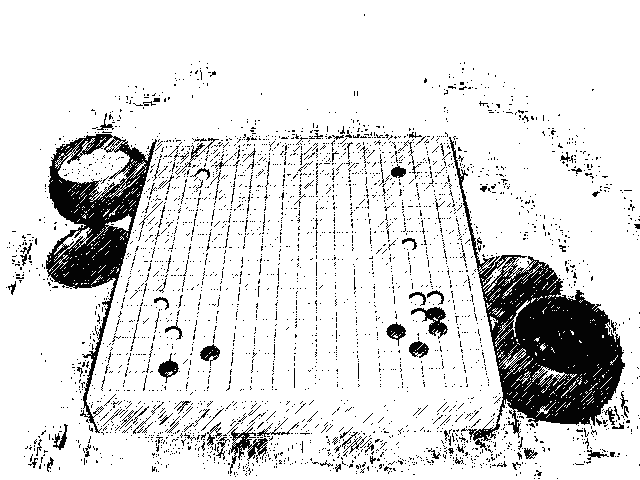
\includegraphics[width=\columnwidth]{board}\vfil}

\columnbreak

\vglue 2cm

{\Large
\centerline{FASCYNUJĄCA GRA PLANSZOWA}
\centerline{Z DALEKIEGO WSCHODU}
}
\vskip 2cm
{\Huge\centerline{GO}}
\vskip 1cm
\centerline{\hskip.7cm\includegraphics{kanji}}

\end{multicols}
\vfill\eject
\end{document}
